
%(BEGIN_QUESTION)
% Copyright 2006, Tony R. Kuphaldt, released under the Creative Commons Attribution License (v 1.0)
% This means you may do almost anything with this work of mine, so long as you give me proper credit

A common analytical sensor used to detect potentially explosive gases (often called a {\it LEL analyzer} in reference to ``Lower Explosive Limit'') is the {\it catalytic combustible gas sensor}.  In this type of sensor, a fine platinum wire is heated by an electric current, and covered by a catalytic substance.  If a mixture of flammable gas(es) and air comes into contact with the sensor, the ensuing combustion will cause the platinum wire to heat up, thus increasing the wire's resistance and signaling the presence of a potentially explosive gas.

In this particular LEL analyzer, two identical platinum wire sensors are connected in series, one of them exposed to a steady stream of sample gas and the other sealed where no gas can reach it.  The voltages dropped by these two resistance elements are digitized by a pair of analog-to-digital converters (ADCs) and interpreted by a microcontroller:

$$\includegraphics[width=15.5cm]{i01592x01.eps}$$

Supposing this circuit is faulty (signaling the presence of explosive gas even when there is no gas present), where would you begin taking diagnostic measurements to isolate the nature of the fault?  Under what sample gas conditions would you prefer to perform these measurements, and why?

\vskip 20pt \vbox{\hrule \hbox{\strut \vrule{} {\bf Suggestions for Socratic discussion} \vrule} \hrule}

\begin{itemize}
\item{} Why do you suppose the two catalytic wire sensors are connected in {\it series}?
\item{} What are the values of some electrical measurements you would expect to see in a ``healthy'' circuit, and what might you expect to see in a circuit where the active gas sensor has failed?  
\item{} What are some component failures that could cause the microcontroller to see a ``hotter'' signal for $R_3$ than for $R_4$?  What effect would this have on gas detection?
\item{} What are some component failures that could cause the microcontroller to see a ``colder'' signal for $R_3$ than for $R_4$?  What effect would this have on gas detection?
\item{} What would happen if resistor $R_1$ were to fail open?
\item{} What would happen if resistor $R_1$ were to fail shorted?
\item{} What would happen if rheostat $R_2$ were to decrease in resistance?
\item{} What would happen if rheostat $R_2$ were to increase in resistance?
\item{} Why do you suppose the sensor's platinum wire is coated with a {\it catalyst}?
\item{} This type of LEL sensor is dependent upon the amount of oxygen present in the gas sample.  Determine the effect that oxygen concentration will have on this type of analyzer (i.e. will an increased oxygen concentration make the instrument ``think'' there is {\it more} or {\it less} flammable gas present?), and then devise a method by which this interference may be compensated.
\end{itemize}

\underbar{file i01592}
%(END_QUESTION)





%(BEGIN_ANSWER)

In a properly operating circuit with no explosive gas present, $V_{R3} = V_{R4}$ or $V_D = 2 V_E$.  I will leave it to you to identify good diagnostic tests!

%(END_ANSWER)





%(BEGIN_NOTES)

In a properly operating circuit with no explosive gas present, $V_{R3} = V_{R4}$ or $V_D = 2 V_E$.  

\vskip 10pt

Use a multimeter to see if $V_{R3} = V_{R4}$.  If the active sensor is failed open, $V_{R3} >> V_{R4}$. 

\vskip 10pt

A condition of $V_{R3} >> V_{R4}$ may exist if $R_3$ fails open {\it or} if $R_4$ fails shorted.  The next diagnostic measurement to take after verifying $V_{R3} >> V_{R4}$ is a voltage measurement across resistor $R_1$: if there is a voltage drop, then there is current in the loop which means $R_4$ has failed shorted.  If there is no voltage drop across $R_1$, then there is no current in the loop which means $R_3$ has failed open.

\vskip 10pt

When performing these diagnostic tests it is recommended you expose the analyzer to a sample with no flammable gases in it, in order to best reveal the fault.  Since the problem here is that the analyzer registers an explosive condition even when none exists, in order to create a scenario that best reveals the problem we must place the analyzer in a condition where it is ``misbehaving''.  By contrast, if there actually were explosive gases present in the analyzer's sample during our diagnostic tests, we may have a difficult time discerning false signs of an explosive condition from real signs of an explosive condition.  

By analogy, imagine an automobile mechanic who is told a car make a certain rattling noise at a certain driving speed.  When diagnosing this noise, the mechanic would be wise to try duplicating the symptom by driving the car at that speed and listening to the rattle itself (identifying features such as its frequency, its location, and its amplitude).  Testing the car while sitting still is unlikely to reveal the fault, except by chance.






\vskip 20pt \vbox{\hrule \hbox{\strut \vrule{} {\bf Virtual Troubleshooting} \vrule} \hrule}

This question is a good candidate for a ``Virtual Troubleshooting'' exercise.  Presenting the diagram to students, you first imagine in your own mind a particular fault in the system.  Then, you present one or more symptoms of that fault (something noticeable by an operator or other user of the system).  Students then propose various diagnostic tests to perform on this system to identify the nature and location of the fault, as though they were technicians trying to troubleshoot the problem.  Your job is to tell them what the result(s) would be for each of the proposed diagnostic tests, documenting those results where all the students can see.

During and after the exercise, it is good to ask students follow-up questions such as:

\begin{itemize}
\item{} What does the result of the last diagnostic test tell you about the fault?
\item{} Suppose the results of the last diagnostic test were different.  What then would that result tell you about the fault?
\item{} Is the last diagnostic test the best one we could do?
\item{} What would be the ideal order of tests, to diagnose the problem in as few steps as possible?
\end{itemize}

%INDEX% Measurement, analytical: catalytic combustible gas sensor
%INDEX% Troubleshooting review: electric circuit diagnostic test usefulness

%(END_NOTES)


